\documentclass[12 pt,a4paper]{report}

\usepackage{amstext}
\usepackage{amsfonts}
\usepackage{graphicx}
\usepackage{amssymb,amsthm,amsmath,amscd}     
\usepackage{latexsym}                         
%\usepackage{enumerate}
\usepackage[ngerman]{babel}
\usepackage[latin1]{inputenc}
%\usepackage{verbatim} fuer Quelltexteingabe

\author{}
\title{}

%Befehle Block--------------------------
%\newcommand{\qed}{\hfill$\square$}

%---------------------------------------
\begin{document}
\setlength\parindent{0pt}

%Titel Seite-----------------------------
\begin{titlepage}
\begin{center}

\vspace*{1.0cm}
\huge
\textsc{\bf{LED-Lenkrad zur Visualisierung der Drehzahl\\
		-\\
    HCI Studio WS 2014/15}}

\vspace*{1.0cm}
\Large
\textsc{Seminararbeit}

\vspace*{3.0cm}
\textsc{
\normalsize{von} \\[0.5\baselineskip]
{\large \ Stefan Vikoler}
}

\vspace*{3.0cm}
\textsc{
\normalsize{Betreuung:\\
Univ.-Prof. Dr. Mag. Manfred Tscheligi\\
Dr. Dipl.-Ing. Alexander Meschtscherjakov}
}

\vspace*{1.0cm}
\textsc{
\normalsize{Universit\"at Salzburg \\
Fachbereich Computerwissenschaften\\
Jakob-Haringer-Stra�e 2\\
A-5020 Salzburg\\
Austria}
}

\end{center}

\end{titlepage}

%Include Block---------------------------
\section*{Abstract}
\itshape
In dieser Seminararbeit wird ein prototypisches LED-Lenkrad zur Visualisierung der Drehzahl in einem Fahrsimulator vorgestellt, welches im Rahmen der Lehrveranstaltung HCI Studio unter dem Thema "`Exploration des Design Spaces 'Lenkrad im Auto'"' unter Aufsicht von Dr. Manfred Tscheligi und Dr. Alexander Meschtscherjakov entstand. Die Arbeit zeigt den Wege der Ideenfindung, dem Design und die Implementierung des Prototypen und die finalen Auswertung der Studienfrage, ob diese Interaktionsmodalit�t von Benutzern favorisiert wird.\\
\upshape

\tableofcontents
\chapter{Einleitung}
Die HCI kann man in viele Aufgabengebiete unterteilen und es gibt auch diverse Definitionen daf�r. Auf jeden Fall beinhaltet die HCI jedoch das Studieren und Entwickeln von verbesserten Arten der User Experience und neuer Interaktionsparadigmen, sowie die Anwendung von interdisziplin�ren Methoden f�r benutzerzentriertes Design. Auch in der Lehrveranstaltung HCI Studio wurde versucht, diese Ziele umzusetzen, indem wir verschiedenste Interaktionskontexte untersuchten, mit dem Ziel diese Kontexte f�r eine optimale Experience zu verbessern und benutzerzentrierte Methoden f�r innovative und optimierte Systeme anzuwenden.\\

Das Thema der Lehrveranstaltung war die Exploration des Design Spaces "`Lenkrad im Auto"' und bestand aus Einzel- und Gruppenaufgaben zu obigem Thema. Ziel war es, durch benutzerzentriertes Design einen innovativen und optimierten Prototypen zu implementieren, welcher den Design Space des Lenkrads im Auto verwendet und das Benutzererlebnis erh�ht.\\

Daf�r klassifizierten wir derzeitige Interaktionsm�glichkeiten am Lenkrad und recherchierten aktuelle Forschungen alternativer Interaktionsm�glichkeiten am Lenkrad. Mit Hilfe der Lehrveranstaltungsleiter, welche uns mit verschiedenen Methoden der Ideenfindung unterst�tzten, konnten wir aus diesen Ergebnissen verschiedene Konzepte erarbeiten, wie man am Lenkrad interagieren k�nnte.\\

In der Gruppe wurde dann eine Interaktionstechnologie fokusiert und jeder setzte das Design und Prototyping von 3 innovative Visualisierungen um. Im Anschluss wurde der Prototyp in Form einer kleinen Nutzerstudie evaluiert.

\chapter{State of the Art}
In der Geschichte der Autoindustrie hat sich im Bereich Fahrer-Cockpit einiges getan und auch die HCI hat �ber die letzten Jahrzehnte User Interfaces im Automobil erforscht. Durch die wachsende Anzahl an Interaktionsm�glichkeiten f�r den Fahrer steigt leider auch die Gefahr, dass dem Fahrer durch die Ablenkung Fehler passieren.\\

Im groben k�nnen die Interaktionsbereiche des Fahrers unterteilt werden in die Windschutzscheibe (z.B. Navi), das Amaturenbrett, die Mittelkonsole, das Lenkrad, dem Boden (z.B. Pedale) und der Peripherie (z.B. Seitenspiegel).\cite{kern} Diese Seminararbeit besch�ftigt sich von nun an im wesentlichen mit der Interaktionsschnittstelle Lenkrad.

\section{Interaktionsm�glichkeiten am Lenkrad}
Die Hauptfunktionalit�t eines Lenkrads ist das Bestimmen der Richtung, in welche sich das Fahrzeug bewegen soll. Daf�r  wird das Lenkrad in die jeweilige Richtung gedreht. Es finden sich jedoch weitere Interaktionsm�glichkeiten am Lenkrad wieder, welche verschiedene Aufgaben erf�llen.\\

So steuert man nicht nur die Richtung, sondern auch andere Funktionalit�ten des Fahrzeuges am Lenkrad an. Man kann beispielsweise die Hupe, Blinker, Lichtanlage, Scheibenwischer, Radio, Sprachsteuerung, Lautsprecheinrichtung, Lautst�rke, Tempomat und weitere Funktionen bet�tigen.\\

Daf�r wurden auch verschiedene Modalit�ten erforscht und eingesetzt, wie diese enorme Anzahl an Aufgaben am effektivsten zu bedienen ist. Das wohl g�ngigste Beispiel ist die Hupe, welche bet�tigt wird indem man in die Mitte des Lenkrads dr�ckt. Weitere Modalit�ten sind zum Beispiel die Hebel links und rechts hinter dem Lenkrad, welche sich oft nach unten, oben, vor und zur�ck dr�cken und im Uhrzeigersinn und gegen den Uhrzeigersinn drehen lassen. Damit werden meist die Lichtanlage, Blinker und Scheibenwischer des Autos bedient. Au�erdem befinden sich heute auch oft noch Kn�pfe auf den Hebeln, um weitere Einstellungen vorzunehmen.

Doch nicht nur Hebel und Druckkn�pfe sondern auch Einstellr�der, Knebelkn�pfed, Drehr�der, etc. finden am Lenkrad eine Einsatzm�glichkeiten.

\section{Related Work}
Die HCI besch�ftigt sich seit langem, wie die gro�e Anzahl an Funktionalit�ten am Lenkrad am effizientesten in Hinsicht Sicherheit, Effektivit�t und Benutzerfreundlichkeit zu bew�ltigen sind. So wurde beispielsweise auch die R�ckseite des Lenkrades in Betracht gezogen und verschiedenen M�glichkeiten vorgestellt diesen Raum zu nutzen.\cite{murer}\\

Ein weiterer Ansatz besch�ftigt sich mit Touch Interfaces und erforscht den Design Space, wie daumengesteuerte Touch Interfaces am besten bedient werden k�nnen.\cite{werner, gonzalez, pfeiffer} Auch mit der Interaktion mittels Sprache und Gesten hat man sich bereits besch�ftigt.\cite{pfleging, doring}

\chapter{Konzepte}
Im Rahmen der Lehrveranstaltung wurden verschiedene Konzepte erarbeitet. Daf�r wurde das Lenkrad zu beginn kritisch betrachtet und es kamen Ideen auf, wie anstatt eines Lenkrads das Fahrzeug mit einem Joystick zu lenken. Oder die Eigenschaften von Lenkrad und Pedalen wurden vertauscht und das Auto wurde mit zwei Pedalen (links und rechts) gelenkt und mit dem Lenkrad - von sich weg dr�ckend (schneller) und zu sich her ziehend (langsamer) - beschleunigt.

Eine weitere Idee war eine Steuerung �hnlich einem Panzer, indem man mit einem Hebel links die beiden linken R�der beschleunigte bzw. verlangsamte und analog einem Hebel rechts hatte.

Einer Idee nach konnte man mit einem Touchpad an der Vorderseite in der Mitte des Lenkrads mittels Symbolen die Blinker, den Radio und weitere Elemente im Auto bedienen.\\

Um f�r weitere Konzepte und Ideen offener zu werden, sollten wir das Lenkrad unter dem Thema Tiere auch exzentrisch betrachten. Dadurch entstanden Erfindungen, ein Auto mit verschiedenen Tierger�uschen zu steuern. So war das Br�llen eines Tigers gleichzusetzen mit dem Bet�tigen des Gaspedals und des Meckern eines Schafes entsprach dem Bremsen. Weiters wurde in einer Idee das Fahrer-Cockpit komplett mit einem gro�en Hamsterrad ersetzte, mit welchem das Fahrzeug gesteuert wurde.\\

Bei der Ideenfindung f�r unseren Prototypen haben wir versucht verschiedene Interfaces miteinzubeziehen. Indem man beispielsweise Funktionen mittels Schiebereglern an der R�ckseite des Lenkrads bet�tigte oder an der Vorderseite ein Touch-Interface befestigt wird, womit man einige Aufgaben durchf�hren kann.

Durchgesetzt hat sich die Idee, Anzeigen im Armaturenbrett und in der Mittelkonsole mittels eines LED-Streifens am �u�eren des Lenkrads zu visualisieren.

\chapter{Design und Implementierung}
Beim Design und der Implementierung des Prototypen stand uns die HCI \& Usability Unit\footnote[1]{https://www.icts.sbg.ac.at/} in Salzburg tatkr�ftig zur Seite. Zum Beispiel konnten wir einen Fahrsimulator dort nutzen. Dieser besteht aus einer Sitzgelegenheit mit zwei Pedalen (Gas und Bremse), samt einem Fanatec Porsche GT3 Lenkrad. An diesem Lenkrad montierten wir am �u�eren Rand einen LED-Streifen in einem transparenten Plastikschlauch und verbanden ihn �ber ein Arduino-Sensor-Board mit dem Fahrsimulator-PC. Auf diesem PC l�uft der OpenSource Fahrsimulator OpenDS\footnote[2]{http://opends.de/}, basierend auf der Programmiersprache Java.\\

Mittels RMI (Remote Method Invocation) konnten wir dann Methoden aus OpenDS abrufen und die r�ckgegebenen Daten am LED-Streifen anzeigen. Diese Seminararbeit beschr�nkt sich darauf, die Drehzahl mittels der LED's darzustellen.\\

Hierf�r wurden drei Methoden entwickelt, die Drehzahl zu Visualisieren.

\section{risingRPM}
Die Methode risingRPM beschreibt eine Visualisierung, in der die LED's von unten nach oben je nach H�he der Drehzahl zu Leuchten beginnen. Au�erdem ver�ndert sich die Farbe von gr�n (niedrige Drehzahl) �ber blau (mittlere Drehzahl) nach rot (hohe Drehzahl).

\section{rpmCicle}
Bei der Methode rpmCicle bewegen sich 10 aufeinander folgende LED's im Uhrzeigersinn rund um das Lenkrad. Die Geschwindigkeit in der die LED's um das Lenkrad kreisen h�ngt von der H�he der Drehzahl im Fahrsimulator ab.

\section{rpmNeedle}
Die Methode rpmNeedle beginnt �hnlich der risingRPM von unten nach oben. Hier jedoch leuchten die LED's nur �ber den linken Rand des Lenkrads und wenn ein Maximum erreicht wird, leuchtet diese LED noch ein paar Sekunden weiter, um dem Benutzer seinen h�chsten RPM-Stand der letzten Sekunden zu visualisieren.\\

\begin{center}
\begin{figure}[ht]
	\centering
  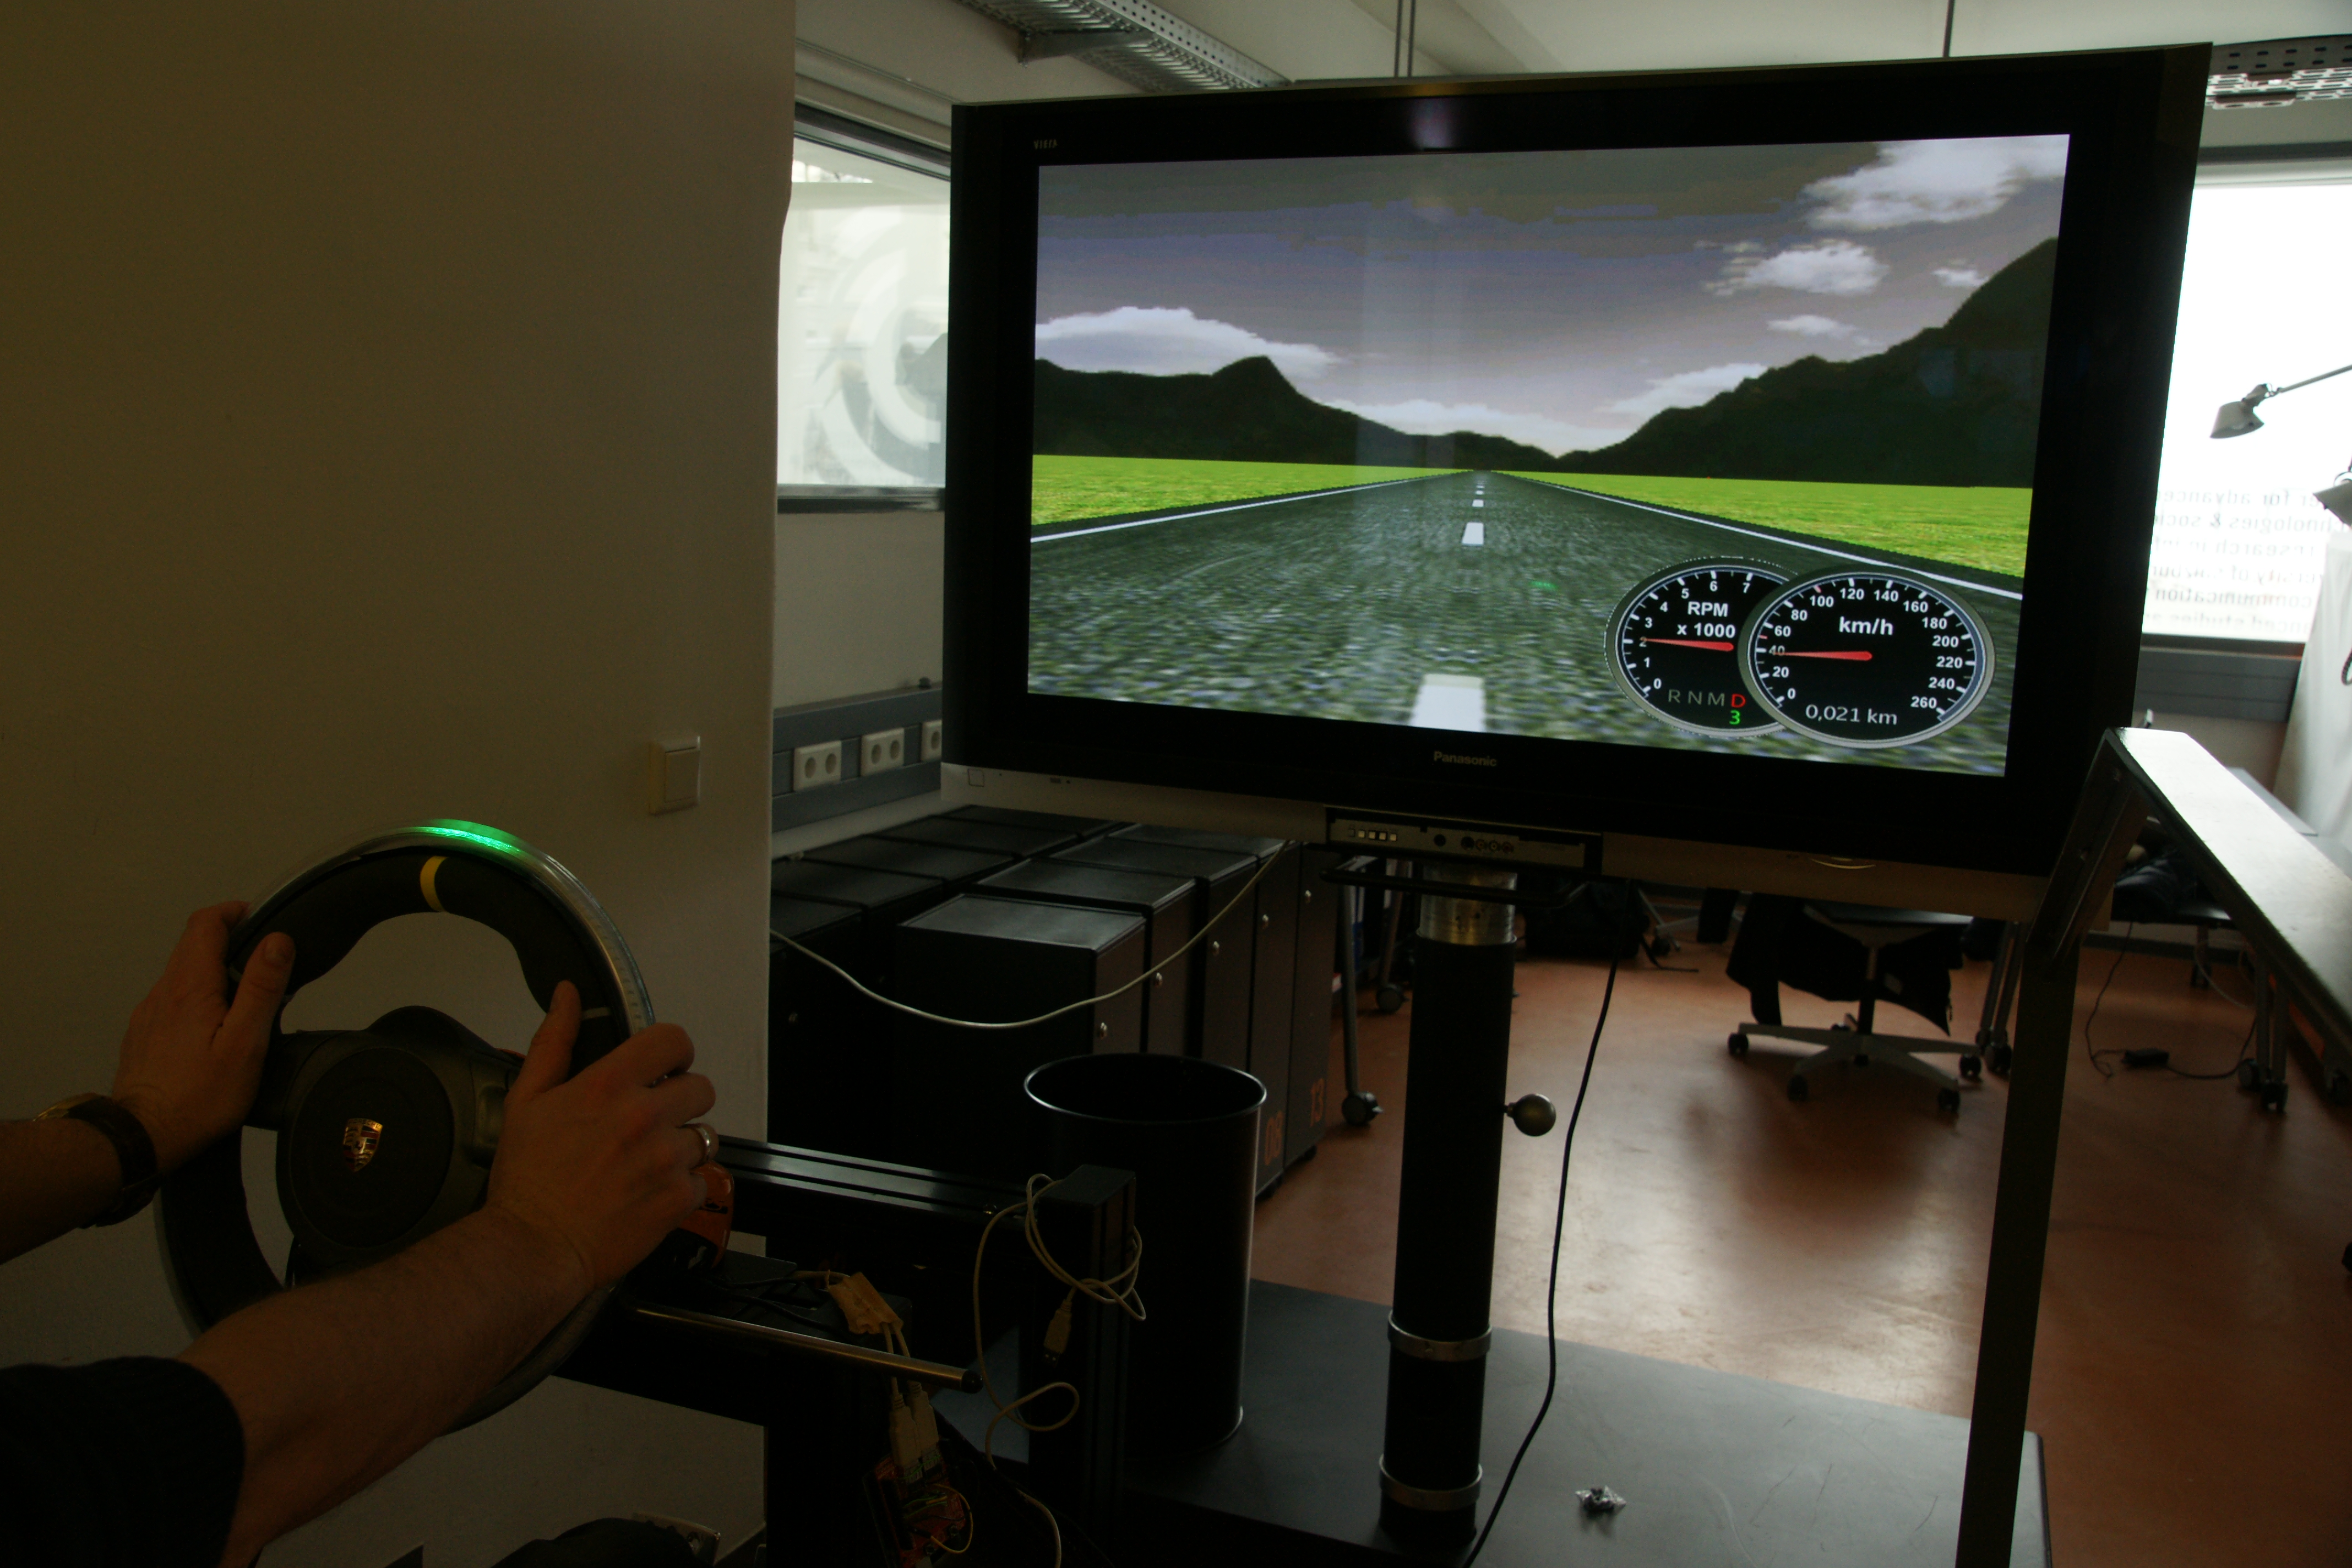
\includegraphics[width=12cm]{abb.jpg}
	\caption{Fahrsimulator Testumgebung mit LED-Lenkrad}
	\label{abb1}
\end{figure}
\end{center}

\chapter{Evaluierung}
Unsere Implementierungen wurden daraufhin anhand einer Nutzerstudie getestet. Daf�r lie�en wir die anderen Lehrveranstaltungsteilnehmer und Mitarbeiter der HCI \& Usability Unit mit dem Fahrsimulator gewisse Strecken fahren und baten sie danach einen kurzen Fragebogen auszuf�llen, um herauszufinden, ob Nutzer diese Technologie privat verwenden w�rden und ob ihnen die Technologie beim Fahren geholfen hat. Dabei wurden folgende sieben Fragen gestellt.
\begin{enumerate}
	\item Ich h�tte das System gerne in meinem Auto
	\item Wenn ich das System in meinem Auto habe, werde ich es benutzen
	\item Die Nutzung des Systems wird meine Fahrleistung verbessern
	\item Ich finde das System ist beim Fahren unpraktisch
	\item Die Nutzung des Systems verbessert meine Bedienung des Autos
	\item Ich finde das System ist beim Fahren n�tzlich
	\item Meine Interaktion mit dem System ist klar verst�ndlich
\end{enumerate}
Diese Fragen konnten mit "`Ich stimme dem 1. Sehr 2. Ziemlich 3. Mittel 4. Wenig 5. nicht zu"' beantwortet werden.\\

Alle drei Visualisierungen wurden hier �hnlich beantwortet und es konnte evaluiert werden, dass die Testuser den Prototyp gerne im Auto h�tten und ihn auch verwenden w�rden. Es war f�r die Tester leicht mit dem System zu interagieren und das System wurde als n�tzlich empfunden. Jedoch konnte der Prototyp keine Verbesserung der Fahrleistung bewirken und auch die Bedienung des Autos wird dadurch nicht vereinfacht. Keine der Testpersonen empfand die Visualisierung als unpraktisch.

\chapter{Reflexion}
Zusammenfassend k�nnen wir aus den Tests schlie�en, dass der Prototyp visuell ansprechend und leicht bedienbar ist. Die Testpersonen waren sehr davon angesprochen, empfanden ihn jedoch nicht als hilfreich bei der eigentlichen Aufgabe, dem Autofahren.\\

Daher kann man den Prototypen gerne als Gadget im Fahrzeug betrachten, der einen gewissen Spa�faktor bringt, aber keine Hilfestellung beim Bedienen des Fahrzeuges bietet.


%----------------------------------------
\bibliographystyle{plain}
\nocite{*}
\bibliography{literatur}
%----------------------------------------
\end{document}